\begin{figure}[htbp]
    \centering
    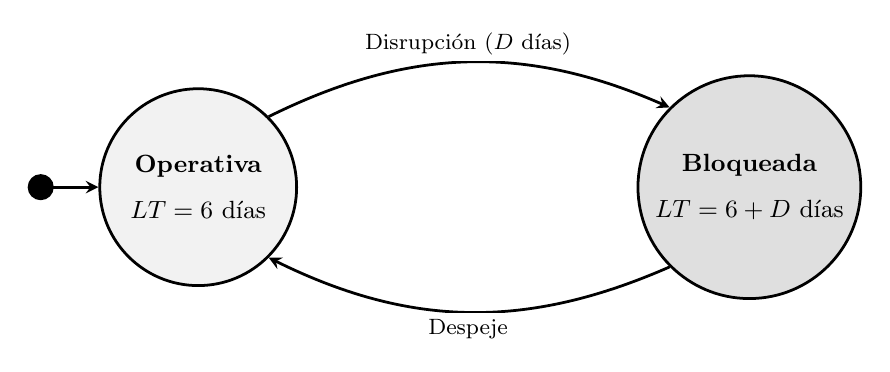
\begin{tikzpicture}[
        font=\small,
        node distance=6cm,
        state/.style={
            circle, draw=black, line width=1pt,
            minimum size=2.5cm,
            text centered, font=\small, align=center
        },
        arrow/.style={->, >=stealth, line width=1pt, bend left=25},
        label/.style={font=\footnotesize, fill=white, inner sep=2pt}
    ]

        % Estados
        \node[state, fill=gray!10] (operativa) at (0,0) {
            \textbf{Operativa}\\[0.2cm]
            $LT = 6$ días
        };

        \node[state, fill=gray!25] (bloqueada) at (7,0) {
            \textbf{Bloqueada}\\[0.2cm]
            $LT = 6 + D$ días
        };

        % Transiciones
        \draw[arrow]
            (operativa.north east) to node[label, above] {
                Disrupción ($D$ días)
            } (bloqueada.north west);

        \draw[arrow]
            (bloqueada.south west) to node[label, below] {
                Despeje
            } (operativa.south east);

        % Estado inicial
        \node[circle, fill=black, minimum size=0.25cm] at (-2,0) {};
        \draw[->, >=stealth, line width=1pt] (-2,0) -- (operativa.west);

    \end{tikzpicture}
    \caption{Máquina de estados de la Ruta 7 (operativa/bloqueada).}
    \label{fig:maquina-estados-ruta}
\end{figure}
